% Created by tikzDevice version 0.12.3 on 2020-01-31 11:45:53
% !TEX encoding = UTF-8 Unicode
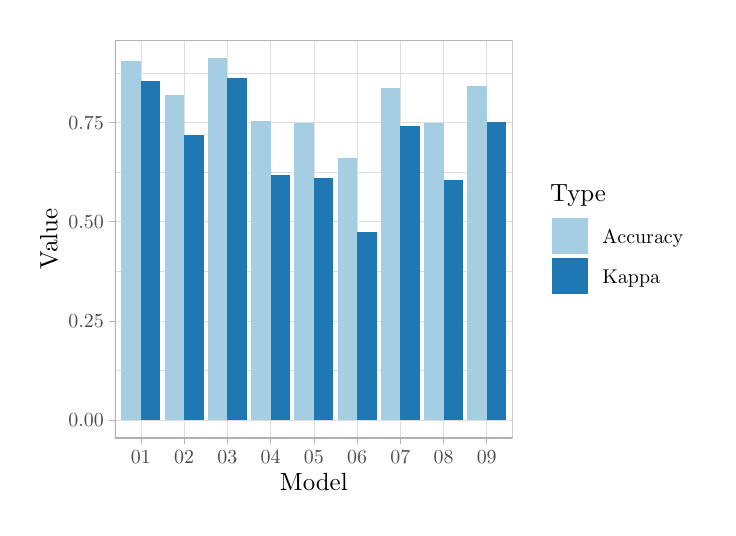
\begin{tikzpicture}[x=1pt,y=1pt]
\definecolor{fillColor}{RGB}{255,255,255}
\path[use as bounding box,fill=fillColor,fill opacity=0.00] (0,0) rectangle (245.72,173.45);
\begin{scope}
\path[clip] (  0.00,  0.00) rectangle (245.72,173.45);
\definecolor{drawColor}{RGB}{255,255,255}
\definecolor{fillColor}{RGB}{255,255,255}

\path[draw=drawColor,line width= 0.5pt,line join=round,line cap=round,fill=fillColor] (  0.00,  0.00) rectangle (245.72,173.45);
\end{scope}
\begin{scope}
\path[clip] ( 31.54, 25.11) rectangle (175.25,168.95);
\definecolor{fillColor}{RGB}{255,255,255}

\path[fill=fillColor] ( 31.54, 25.11) rectangle (175.25,168.95);
\definecolor{drawColor}{gray}{0.87}

\path[draw=drawColor,line width= 0.1pt,line join=round] ( 31.54, 49.56) --
	(175.25, 49.56);

\path[draw=drawColor,line width= 0.1pt,line join=round] ( 31.54, 85.40) --
	(175.25, 85.40);

\path[draw=drawColor,line width= 0.1pt,line join=round] ( 31.54,121.23) --
	(175.25,121.23);

\path[draw=drawColor,line width= 0.1pt,line join=round] ( 31.54,157.07) --
	(175.25,157.07);

\path[draw=drawColor,line width= 0.2pt,line join=round] ( 31.54, 31.64) --
	(175.25, 31.64);

\path[draw=drawColor,line width= 0.2pt,line join=round] ( 31.54, 67.48) --
	(175.25, 67.48);

\path[draw=drawColor,line width= 0.2pt,line join=round] ( 31.54,103.31) --
	(175.25,103.31);

\path[draw=drawColor,line width= 0.2pt,line join=round] ( 31.54,139.15) --
	(175.25,139.15);

\path[draw=drawColor,line width= 0.2pt,line join=round] ( 40.92, 25.11) --
	( 40.92,168.95);

\path[draw=drawColor,line width= 0.2pt,line join=round] ( 56.54, 25.11) --
	( 56.54,168.95);

\path[draw=drawColor,line width= 0.2pt,line join=round] ( 72.16, 25.11) --
	( 72.16,168.95);

\path[draw=drawColor,line width= 0.2pt,line join=round] ( 87.78, 25.11) --
	( 87.78,168.95);

\path[draw=drawColor,line width= 0.2pt,line join=round] (103.40, 25.11) --
	(103.40,168.95);

\path[draw=drawColor,line width= 0.2pt,line join=round] (119.02, 25.11) --
	(119.02,168.95);

\path[draw=drawColor,line width= 0.2pt,line join=round] (134.64, 25.11) --
	(134.64,168.95);

\path[draw=drawColor,line width= 0.2pt,line join=round] (150.26, 25.11) --
	(150.26,168.95);

\path[draw=drawColor,line width= 0.2pt,line join=round] (165.88, 25.11) --
	(165.88,168.95);
\definecolor{fillColor}{RGB}{31,120,180}

\path[fill=fillColor] ( 40.92, 31.64) rectangle ( 47.95,154.08);
\definecolor{fillColor}{RGB}{166,206,227}

\path[fill=fillColor] ( 33.89, 31.64) rectangle ( 40.92,161.57);
\definecolor{fillColor}{RGB}{31,120,180}

\path[fill=fillColor] ( 56.54, 31.64) rectangle ( 63.57,134.53);
\definecolor{fillColor}{RGB}{166,206,227}

\path[fill=fillColor] ( 49.51, 31.64) rectangle ( 56.54,149.00);
\definecolor{fillColor}{RGB}{31,120,180}

\path[fill=fillColor] ( 72.16, 31.64) rectangle ( 79.19,155.32);
\definecolor{fillColor}{RGB}{166,206,227}

\path[fill=fillColor] ( 65.13, 31.64) rectangle ( 72.16,162.41);
\definecolor{fillColor}{RGB}{31,120,180}

\path[fill=fillColor] ( 87.78, 31.64) rectangle ( 94.81,120.25);
\definecolor{fillColor}{RGB}{166,206,227}

\path[fill=fillColor] ( 80.75, 31.64) rectangle ( 87.78,139.78);
\definecolor{fillColor}{RGB}{31,120,180}

\path[fill=fillColor] (103.40, 31.64) rectangle (110.43,119.13);
\definecolor{fillColor}{RGB}{166,206,227}

\path[fill=fillColor] ( 96.37, 31.64) rectangle (103.40,138.94);
\definecolor{fillColor}{RGB}{31,120,180}

\path[fill=fillColor] (119.02, 31.64) rectangle (126.05, 99.74);
\definecolor{fillColor}{RGB}{166,206,227}

\path[fill=fillColor] (111.99, 31.64) rectangle (119.02,126.37);
\definecolor{fillColor}{RGB}{31,120,180}

\path[fill=fillColor] (134.64, 31.64) rectangle (141.67,138.00);
\definecolor{fillColor}{RGB}{166,206,227}

\path[fill=fillColor] (127.61, 31.64) rectangle (134.64,151.51);
\definecolor{fillColor}{RGB}{31,120,180}

\path[fill=fillColor] (150.26, 31.64) rectangle (157.29,118.25);
\definecolor{fillColor}{RGB}{166,206,227}

\path[fill=fillColor] (143.23, 31.64) rectangle (150.26,138.94);
\definecolor{fillColor}{RGB}{31,120,180}

\path[fill=fillColor] (165.88, 31.64) rectangle (172.91,139.20);
\definecolor{fillColor}{RGB}{166,206,227}

\path[fill=fillColor] (158.85, 31.64) rectangle (165.88,152.35);
\definecolor{drawColor}{gray}{0.70}

\path[draw=drawColor,line width= 0.5pt,line join=round,line cap=round] ( 31.54, 25.11) rectangle (175.25,168.95);
\end{scope}
\begin{scope}
\path[clip] (  0.00,  0.00) rectangle (245.72,173.45);
\definecolor{drawColor}{gray}{0.30}

\node[text=drawColor,anchor=base east,inner sep=0pt, outer sep=0pt, scale=  0.72] at ( 27.49, 29.17) {0.00};

\node[text=drawColor,anchor=base east,inner sep=0pt, outer sep=0pt, scale=  0.72] at ( 27.49, 65.00) {0.25};

\node[text=drawColor,anchor=base east,inner sep=0pt, outer sep=0pt, scale=  0.72] at ( 27.49,100.83) {0.50};

\node[text=drawColor,anchor=base east,inner sep=0pt, outer sep=0pt, scale=  0.72] at ( 27.49,136.67) {0.75};
\end{scope}
\begin{scope}
\path[clip] (  0.00,  0.00) rectangle (245.72,173.45);
\definecolor{drawColor}{gray}{0.70}

\path[draw=drawColor,line width= 0.2pt,line join=round] ( 29.29, 31.64) --
	( 31.54, 31.64);

\path[draw=drawColor,line width= 0.2pt,line join=round] ( 29.29, 67.48) --
	( 31.54, 67.48);

\path[draw=drawColor,line width= 0.2pt,line join=round] ( 29.29,103.31) --
	( 31.54,103.31);

\path[draw=drawColor,line width= 0.2pt,line join=round] ( 29.29,139.15) --
	( 31.54,139.15);
\end{scope}
\begin{scope}
\path[clip] (  0.00,  0.00) rectangle (245.72,173.45);
\definecolor{drawColor}{gray}{0.70}

\path[draw=drawColor,line width= 0.2pt,line join=round] ( 40.92, 22.86) --
	( 40.92, 25.11);

\path[draw=drawColor,line width= 0.2pt,line join=round] ( 56.54, 22.86) --
	( 56.54, 25.11);

\path[draw=drawColor,line width= 0.2pt,line join=round] ( 72.16, 22.86) --
	( 72.16, 25.11);

\path[draw=drawColor,line width= 0.2pt,line join=round] ( 87.78, 22.86) --
	( 87.78, 25.11);

\path[draw=drawColor,line width= 0.2pt,line join=round] (103.40, 22.86) --
	(103.40, 25.11);

\path[draw=drawColor,line width= 0.2pt,line join=round] (119.02, 22.86) --
	(119.02, 25.11);

\path[draw=drawColor,line width= 0.2pt,line join=round] (134.64, 22.86) --
	(134.64, 25.11);

\path[draw=drawColor,line width= 0.2pt,line join=round] (150.26, 22.86) --
	(150.26, 25.11);

\path[draw=drawColor,line width= 0.2pt,line join=round] (165.88, 22.86) --
	(165.88, 25.11);
\end{scope}
\begin{scope}
\path[clip] (  0.00,  0.00) rectangle (245.72,173.45);
\definecolor{drawColor}{gray}{0.30}

\node[text=drawColor,anchor=base,inner sep=0pt, outer sep=0pt, scale=  0.72] at ( 40.92, 16.10) {01};

\node[text=drawColor,anchor=base,inner sep=0pt, outer sep=0pt, scale=  0.72] at ( 56.54, 16.10) {02};

\node[text=drawColor,anchor=base,inner sep=0pt, outer sep=0pt, scale=  0.72] at ( 72.16, 16.10) {03};

\node[text=drawColor,anchor=base,inner sep=0pt, outer sep=0pt, scale=  0.72] at ( 87.78, 16.10) {04};

\node[text=drawColor,anchor=base,inner sep=0pt, outer sep=0pt, scale=  0.72] at (103.40, 16.10) {05};

\node[text=drawColor,anchor=base,inner sep=0pt, outer sep=0pt, scale=  0.72] at (119.02, 16.10) {06};

\node[text=drawColor,anchor=base,inner sep=0pt, outer sep=0pt, scale=  0.72] at (134.64, 16.10) {07};

\node[text=drawColor,anchor=base,inner sep=0pt, outer sep=0pt, scale=  0.72] at (150.26, 16.10) {08};

\node[text=drawColor,anchor=base,inner sep=0pt, outer sep=0pt, scale=  0.72] at (165.88, 16.10) {09};
\end{scope}
\begin{scope}
\path[clip] (  0.00,  0.00) rectangle (245.72,173.45);
\definecolor{drawColor}{RGB}{0,0,0}

\node[text=drawColor,anchor=base,inner sep=0pt, outer sep=0pt, scale=  0.90] at (103.40,  6.25) {Model};
\end{scope}
\begin{scope}
\path[clip] (  0.00,  0.00) rectangle (245.72,173.45);
\definecolor{drawColor}{RGB}{0,0,0}

\node[text=drawColor,rotate= 90.00,anchor=base,inner sep=0pt, outer sep=0pt, scale=  0.90] at ( 10.70, 97.03) {Value};
\end{scope}
\begin{scope}
\path[clip] (  0.00,  0.00) rectangle (245.72,173.45);
\definecolor{fillColor}{RGB}{255,255,255}

\path[fill=fillColor] (184.25, 71.85) rectangle (241.22,122.21);
\end{scope}
\begin{scope}
\path[clip] (  0.00,  0.00) rectangle (245.72,173.45);
\definecolor{drawColor}{RGB}{0,0,0}

\node[text=drawColor,anchor=base west,inner sep=0pt, outer sep=0pt, scale=  0.90] at (188.75,110.63) {Type};
\end{scope}
\begin{scope}
\path[clip] (  0.00,  0.00) rectangle (245.72,173.45);
\definecolor{fillColor}{RGB}{255,255,255}

\path[fill=fillColor] (188.75, 90.80) rectangle (203.21,105.26);
\end{scope}
\begin{scope}
\path[clip] (  0.00,  0.00) rectangle (245.72,173.45);
\definecolor{fillColor}{RGB}{166,206,227}

\path[fill=fillColor] (189.46, 91.51) rectangle (202.49,104.55);
\end{scope}
\begin{scope}
\path[clip] (  0.00,  0.00) rectangle (245.72,173.45);
\definecolor{fillColor}{RGB}{255,255,255}

\path[fill=fillColor] (188.75, 76.35) rectangle (203.21, 90.80);
\end{scope}
\begin{scope}
\path[clip] (  0.00,  0.00) rectangle (245.72,173.45);
\definecolor{fillColor}{RGB}{31,120,180}

\path[fill=fillColor] (189.46, 77.06) rectangle (202.49, 90.09);
\end{scope}
\begin{scope}
\path[clip] (  0.00,  0.00) rectangle (245.72,173.45);
\definecolor{drawColor}{RGB}{0,0,0}

\node[text=drawColor,anchor=base west,inner sep=0pt, outer sep=0pt, scale=  0.72] at (207.71, 95.55) {Accuracy};
\end{scope}
\begin{scope}
\path[clip] (  0.00,  0.00) rectangle (245.72,173.45);
\definecolor{drawColor}{RGB}{0,0,0}

\node[text=drawColor,anchor=base west,inner sep=0pt, outer sep=0pt, scale=  0.72] at (207.71, 81.10) {Kappa};
\end{scope}
\end{tikzpicture}
